

We evaluate our custom compression scheme against Morden, Ropsten and Frontier blockchains.
\paragraph{Ropsten}
Ropsten is the latest private blockchain aimed as a testnet for the \eth{} developers. It was launched recently and therefore has fewer transactions but characterizes the main blockchain fairly well.\footnote{Launched on Nov 20, 2016.}
It has about 120K blocks and 170K transactions of which 8.5K (about 5\%) create new contracts.
Occupying a size of about 100MB, this is the smallest blockchain in our evaluation. 
\paragraph{Frontier}
Frontier is the main \eth{} blockchain and occupies around 3.5GB. It has 3M blocks and 13M transactions of which 225K (about 1.7\%) create transactions. 
This is the largest blockchain in our evaluation.

\paragraph{Morden}
Morden is a private blockchain serving as a testnet since the start of \eth{} blockchain. 
It has about 1.9M blocks and 5M transactions of which 108K (about 2 \%) create new contracts. The entire blockchain occupies about 2.1GB.

\begin{table*}[!b]
\centering
\captionsetup{justification=centering}
\begin{tabular}{ >{\bfseries}c| p{2cm} | p{2cm} |p{2cm} | p{1.5cm} | p{1.5cm} }
	Program & {Compressed Size of Original File (MB)} & {Compressed Size on Custom format (MB)} & {Compressed Size on Custom format with Huffman Encoding (MB)}& Percentage Gain without Huffman Encoding & Percentage Gain with Huffman Encoding\\
  \hline
  gzip  & 33.4 & 27.5 & 29.4 & 17.7 & 12.0 \\
  bzip2 & 31.0 & 26.7 & 28.6 & 13.9 & 7.8  \\
  xz   & 27.8 & 22.4 &  23.3 & 19.4 & 16.2 \\
\end{tabular}
\caption{Compression of Ropsten testnet. \\ Original Size = 98.6MB. Custom format size = 47.8MB}
\label{tab:compropsten}
\end{table*}

\FloatBarrier
Table \ref{tab:origvscustom} shows the compression gains obtained after using our technique.
As can be seen, savings as much as 40\% can be seen on the main blockchain demonstrating the usefulness
of our technique.

As mentioned earlier, we do not aim to compete against the existing compressing tools that are mature.
However, we provide a comparative evaluation of our tool against gzip, bzip2 and xz. 

Table~\ref{tab:compropsten} 
shows the additional compression savings that were possible by compressing 
our custom format for Ropsten using gzip, bzip2 and xz.

Table~\ref{tab:compmorden} 
shows the additional compression savings that were possible by compressing 
our custom format for Morden using gzip, bzip2 and xz.

Table~\ref{tab:compfrontier} 
shows the additional compression savings that were possible by compressing 
our custom format for Frontier  using gzip, bzip2 and xz.




\begin{table*}[!t]
\centering
\captionsetup{justification=centering}
\begin{tabular}{ >{\bfseries}c| p{2cm} | p{2cm} | p{2cm} | p{1.5cm} | p{1.5cm} }
	Program & {Compressed Size of Original File (MB)} & {Compressed Size on Custom format (MB)} & {Compressed Size on Custom format with Huffman Encoding (MB)} & Percentage Gain without Huffman Encoding & Percentage Gain with Huffman Encoding \\
  \hline
  gzip  & 812.2 & 701.3 & 739.6 & 13.7 & 9.0 \\
  bzip2 & 762.9 & 685.6 & 725.8 & 10.1 & 5.0 \\
  xz   & 686.7 & 599.2 &  620.7 & 12.7 & 9.6 \\
\end{tabular}
\caption{Compression of Morden testnet. \\Original Size = 2160MB. Custom format size = 1135.4MB}
\label{tab:compmorden}
\end{table*}

\begin{table*}[!b]
	\centering
\captionsetup{justification=centering}
\begin{tabular}{ >{\bfseries}c| p{2cm} | p{2cm} | p{2cm} | p{1.5cm} | p{1.5cm} }
	Program & {Compressed Size of Original File (MB)} & {Compressed Size on Custom format without Huffman Encoding (MB)} & {Compressed Size on Custom format with Huffman Encoding (MB)} &Percentage Gain without Huffman Encoding & Percentage Gain with Huffman Encoding\\
  \hline
  gzip  & 1807.1 & 1481.1 & 1627.9 & 18.0 & 10.1 \\
  bzip2 & 1751.3 & 1474.6 & 1590.0 & 15.8 & 9.2 \\
  xz   & 1541.8 & 1367.6 & 1398.7 & 11.3  & 9.3 \\
\end{tabular}
\caption{Compression of Frontier mainnet. \\ Original Size = 3434.6MB. Custom format size = 2069MB}
\label{tab:compfrontier}
\end{table*}

We summarize the additional compression gains for each compression scheme in Figure~\ref{fig:gzip}, Figure~\ref{fig:bzip2} and Figure~\ref{fig:xz}. 
As we can see, the results are encouraging and show room for improvement.

\pagebreak
\begin{figure}
	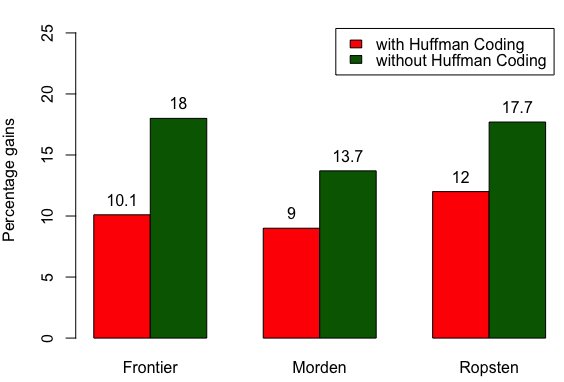
\includegraphics[scale=0.45]{plots/gzip}
	\caption{Additional compression gains (\%) using gzip}
	\label{fig:gzip}
\end{figure}
\begin{figure}
	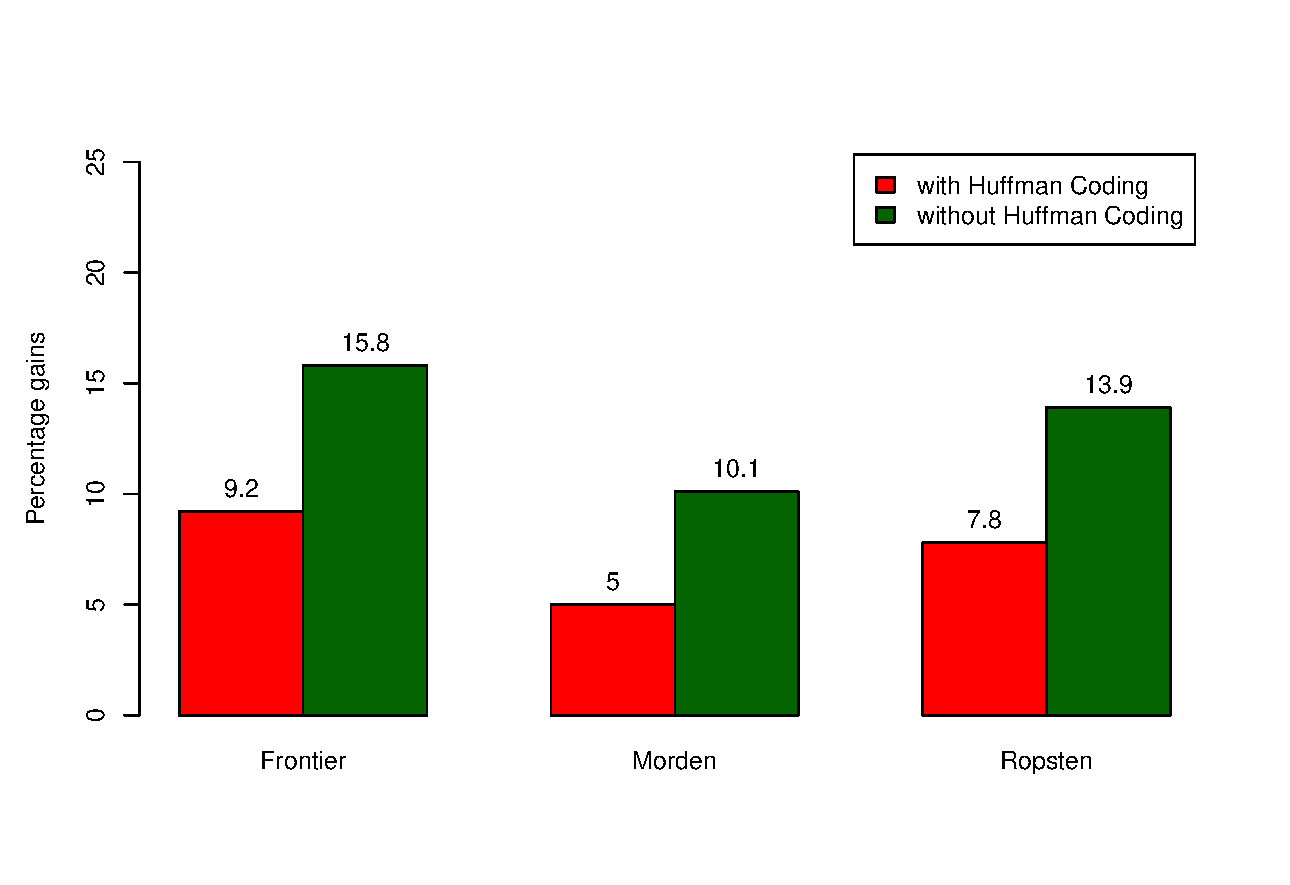
\includegraphics[scale=0.45]{plots/bzip2}
	\caption{Additional compression gains (\%) using bzip2}
	\label{fig:bzip2}
\end{figure}
\begin{figure}
	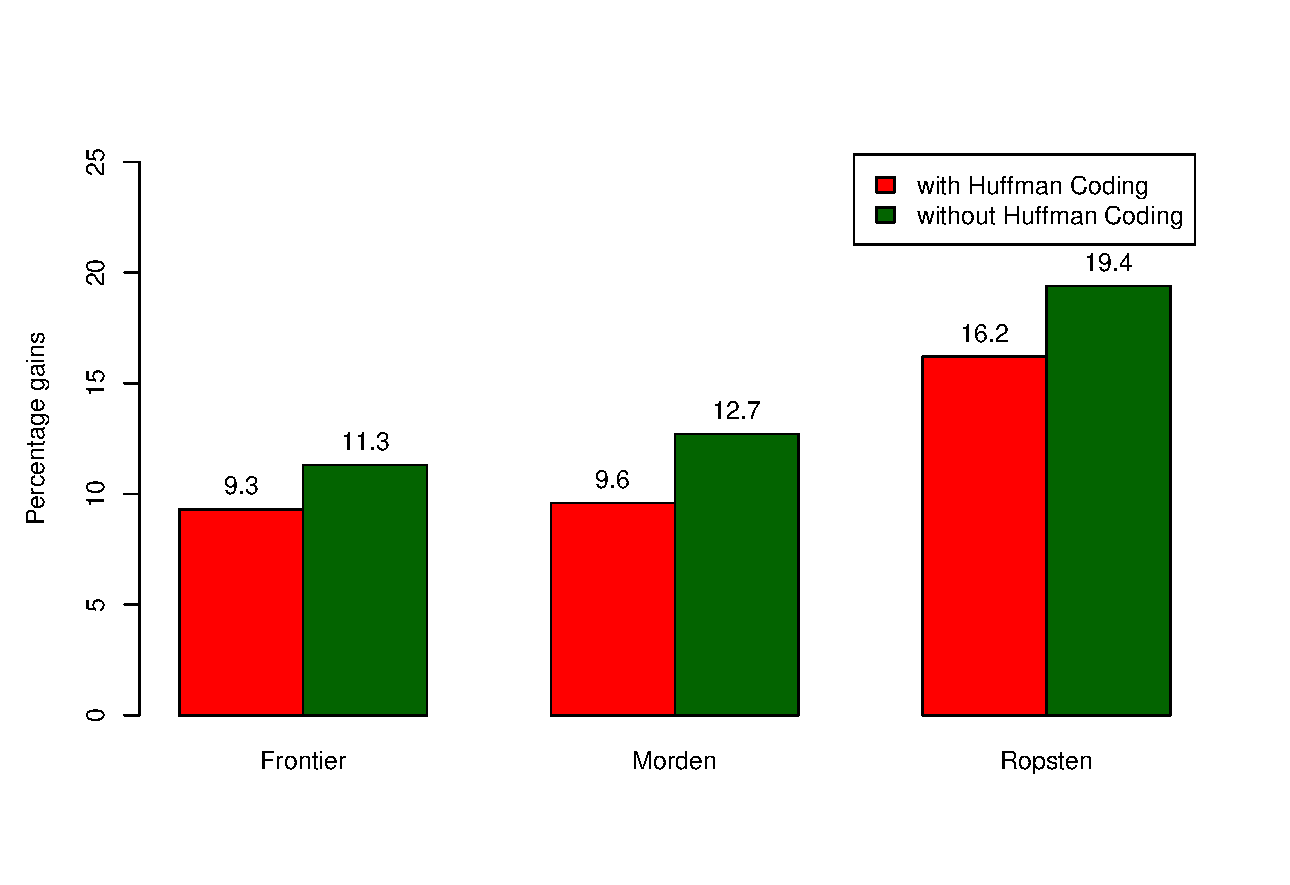
\includegraphics[scale=0.45]{plots/xz}
	\caption{Additional compression gains (\%) using xz}
	\label{fig:xz}
\end{figure}

To demonstrate the feasibility of our approach, we also measure the compression time. 
For brevity, we only 
present the values for compressing Morden blockchain.
The runtime performance of our tool is proportional to the total number of blocks and transactions. 
To generate the custom format without Huffman encoding, it takes about 150 seconds to generate the custom format and with Huffman encoding it takes about 250 seconds. 


Table~\ref{tab:comptime} compares the time taken to compress the binaries before and after applying our technique. As expected, it is less for binaries that are in custom format. 
To make a fair comparison, we should also include the time taken to create the custom format i.e., 150 and 250 seconds depending on whether Huffman encoding is turned on.
Note that our tool is a prototype and is not optimized for runtime performance. 
Yet, the performance is comparable. 
In fact, it outperforms in the case of xz which is encouraging.
Figure~\ref{comptime} shows the same graphically. The dotted green and blue lines show the compression with and without our tool
overheads. In case of xz the total compression time (including the overhead) is about half the original one.


\begin{table}[H]
	\centering
	\begin{tabular}{c | p{1.cm} | p{1.5cm}} 
	Program & {Original Compression Time} & {Compression Time using our custom format} \\
	\hline
	gzip & 220  & 71 \\
	bzip2 & 360  & 245\\
	xz & 1340 & 520 \\
	\end{tabular}
	\caption{Compression time in seconds}
	\label{tab:comptime}
\end{table}
\begin{figure}
	\centering
	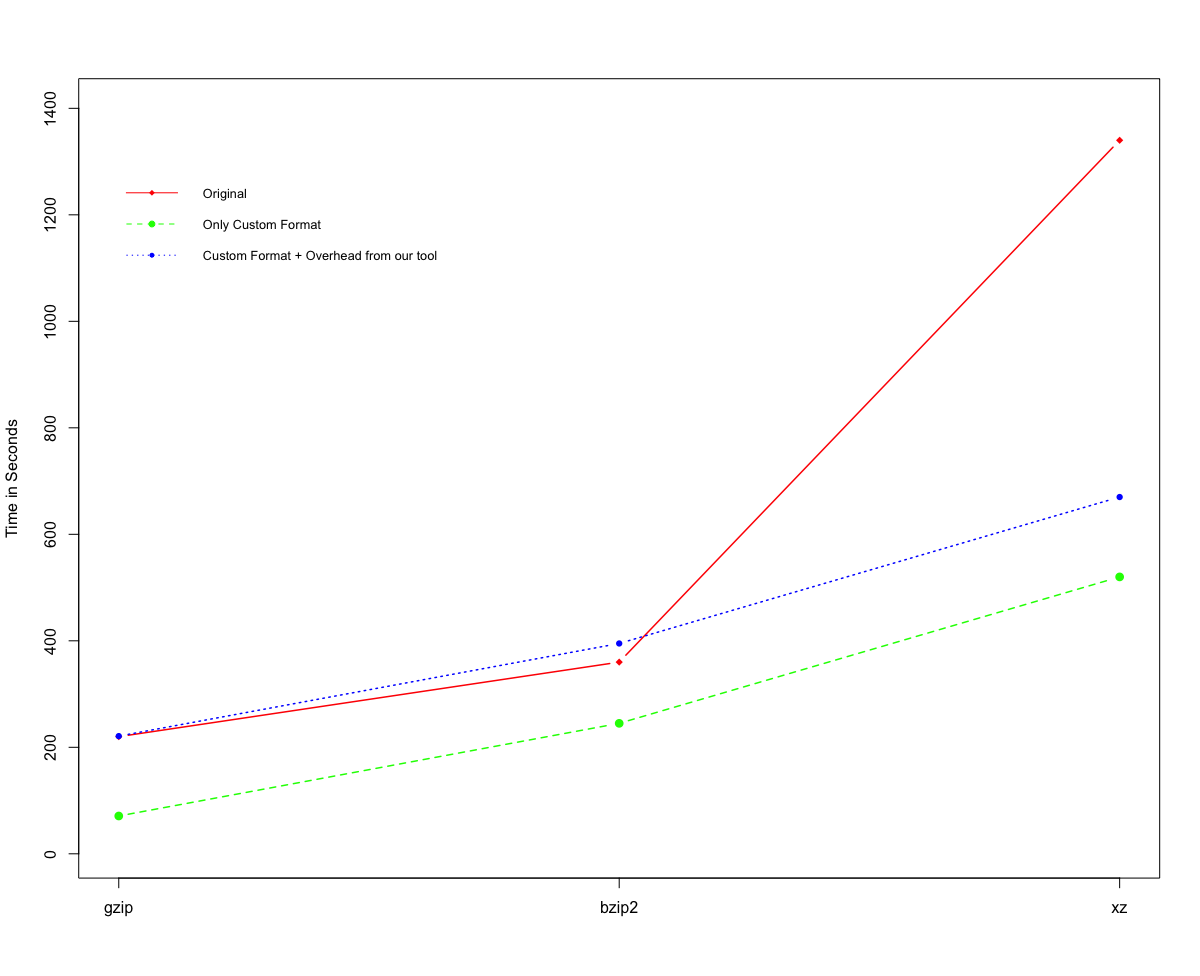
\includegraphics[width=\textwidth]{plots/time}
	\caption{Compression time in seconds}
	\label{fig:comptime}
\end{figure}
